\documentclass[tikz,border=4pt]{standalone}
\usepackage{fontspec}
\setsansfont{Latin Modern Sans}
\usepackage[none]{hyphenat}
\usetikzlibrary{positioning,arrows.meta,shapes.geometric}
\begin{document}
\sffamily\footnotesize
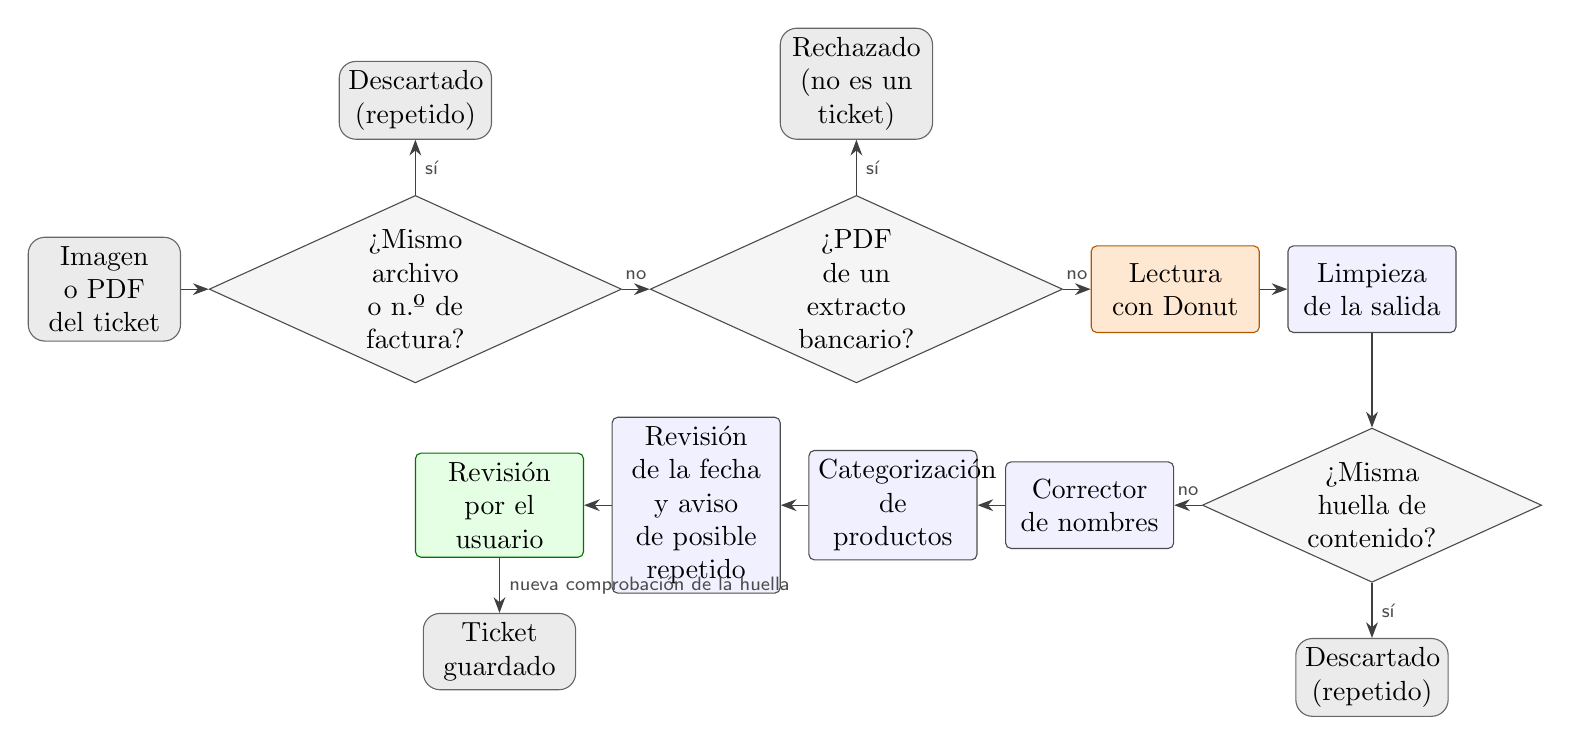
\begin{tikzpicture}[
  node distance=5mm and 3.5mm,
  paso/.style={draw=black!70, rounded corners=2pt, fill=blue!6, align=center, minimum height=11mm, text width=19mm},
  modelo/.style={paso, fill=orange!18, draw=orange!70!black},
  decision/.style={draw=black!70, diamond, aspect=2.2, fill=black!4, align=center, inner sep=1pt, text width=17mm},
  fin/.style={draw=black!60, rounded corners=6pt, fill=black!8, align=center, text width=17mm, minimum height=8mm},
  flecha/.style={-{Stealth[length=2mm]}, black!75},
  etiqueta/.style={font=\sffamily\scriptsize, black!70}]
% Fila 1
\node[fin] (subida) {Imagen o PDF del ticket};
\node[decision, right=of subida] (hash) {¿Mismo archivo o n.º de factura?};
\node[decision, right=of hash] (extracto) {¿PDF de un extracto bancario?};
\node[modelo, right=of extracto] (donut) {Lectura con Donut};
\node[paso, right=of donut] (limpia) {Limpieza de la salida};
% Fila 2
\node[decision, below=12mm of limpia] (huella) {¿Misma huella de contenido?};
\node[paso, left=of huella] (corrector) {Corrector de nombres};
\node[paso, left=of corrector] (categ) {Categorización de productos};
\node[paso, left=of categ] (fecha) {Revisión de la fecha y aviso de posible repetido};
\node[paso, left=of fecha, fill=green!10, draw=green!45!black] (revision) {Revisión por el usuario};
\node[fin, below=7mm of revision] (guardar) {Ticket guardado};
\node[fin, above=7mm of hash, text width=17mm] (descartado) {Descartado (repetido)};
\node[fin, above=7mm of extracto, text width=17mm] (rechazado) {Rechazado (no es un ticket)};
\node[fin, below=7mm of huella, text width=17mm] (descartado2) {Descartado (repetido)};
% Flechas
\draw[flecha] (subida) -- (hash);
\draw[flecha] (hash) -- node[above, etiqueta]{no} (extracto);
\draw[flecha] (extracto) -- node[above, etiqueta]{no} (donut);
\draw[flecha] (donut) -- (limpia);
\draw[flecha] (limpia) -- (huella);
\draw[flecha] (huella) -- node[above, etiqueta]{no} (corrector);
\draw[flecha] (corrector) -- (categ);
\draw[flecha] (categ) -- (fecha);
\draw[flecha] (fecha) -- (revision);
\draw[flecha] (revision) -- node[right, etiqueta]{nueva comprobación de la huella} (guardar);
\draw[flecha] (hash) -- node[right, etiqueta]{sí} (descartado);
\draw[flecha] (extracto) -- node[right, etiqueta]{sí} (rechazado);
\draw[flecha] (huella) -- node[right, etiqueta]{sí} (descartado2);
\end{tikzpicture}
\end{document}
